\chapter{Selection}
\label{ref:sel}

This chapter describes the selection procedure for samples used in this
analysis which involves an online and offline selection.
The initial online selection are a composition of
pre-defined triggers and cuts provided by the LHCb experiment;
some of them may be limiting so extra care is needed to avoid biasing important
physical quantities.
The follow-up offline selection are entirely imposed by analysts
to further balance signal selection and background rejection efficiencies
and separate the signal-like sample from various backgrounds.

Most of the samples are directly used in building fit templates;
the selection procedure for these are discussed in \cref{ref:sel:data} and
\cref{ref:sel:mc}.
Selection of samples used in auxiliary studies is discussed in
\cref{ref:sel:aux-study}.
Additional technologies are used in the selection process;
these are described in more details in
\cref{ref:sel:tech}.


\section{Data samples}
\label{ref:sel:data}

This analysis currently uses 1665~pb$^{-1}$ of proton-proton collision data
recorded by LHCb in 2016 at $\sqrt{s} = 13$~TeV.
It is planned to extend the analysis to employ data taken in the full
2016--2018 period (run 2).
The rest of the section describes selection procedures for various data samples,
which are:

\begin{itemize}
    \item \nameref{ref:sel:data:rs}:
        the nominal data samples to be fitted.
    \item \nameref{ref:sel:data:ws}:
        for characterizing various combinatorial backgrounds
        which are random combinations of the \DXmu pairs that are \emph{not}
        originating from the same $B$ decay but pass the selections
        requiring so.
    \item \nameref{ref:sel:data:fake-mu}:
        for studying the contributions from other charged particles
        mis-identified as muon in the nominal data sample.
\end{itemize}


\subsection{Right-sign samples}
\label{ref:sel:data:rs}

These are the data samples used in the fit where the signal and normalization
yields are extracted.
The samples contain right-sign \DXmu pairs,
the pairs that have the correct charges to form a legitimate $B$ meson.
That is, only \Dz\mun and \Dstarp\mun (and their charge conjugates).
The \muon in these samples are required to pass \muon particle identification
(PID) requirements.

The online selection for the \Dz\mun and \Dstarp\mun final states,
henceforth referred as \Dz channel and \Dstar channel,
are identical.
The selection involves an online trigger path:
a composition of hardware (L0) and software triggers (HLT1, HLT2),
as listed in \cref{tab:triggers}.
Overall, the online selection requires a \muon candidate to form
a well-defined vertex
with a high $p_T$ $\Dz (\rightarrow \Km \pip)$ candidate,
requiring both particles to be close to each other and are not directly coming
from the primary $pp$ decay vertex (PV).
More details about the trigger path are given below.


\begin{table}[!htb]
    \caption{
        Trigger path for this analysis.
        For terminologies such as TIS and TOS, refer to
        \cref{appx:trigger-cat}.
    }
    \label{tab:triggers}
    \centering
    \parnotereset
    \begin{tabular}{c|c}
        \toprule
        {\bf Trigger level} & {\bf Requirements} \\
        \midrule
        L0 & \Dz L0Hadron TOS || \B L0Global TIS \\
        HLT1 & \makecell{
            (\kaon~\smalltt{Hlt1TrackMVA} TOS || \pion~\smalltt{Hlt1TrackMVA} TOS)\parnote{
                This is almost equivalent to \Dz~\smalltt{Hlt1TrackMVA} TOS, with a
                $\sim\!0.0027\%$ difference in selected events in
                reconstructed data sample in \Dz channel.
                Henceforth these two trigger paths are considered equivalent.
            } || \\ \Dz~\smalltt{Hlt1TwoTrackMVA} TOS
        } \\
        HLT2 & \B~\smalltt{Hlt2XcMuXForTauB2XcMu} TOS \\
        \bottomrule
    \end{tabular}
    \begin{flushleft}
        \parnotes
    \end{flushleft}
\end{table}


%%%%
The L0 triggers are chosen to make sure events are not trigged by
the \muon track \emph{alone} which would introduce a \pt bias\footnote{
    According to table 1 in \cite{LHCb-DP-2019-001},
    the minimum \pt threshold across all L0 triggers is 1.35 GeV for 2018
    L0Muon trigger.
} on the \muon.
Such a bias is very problematic for this analysis as \muon from signal
$\tauon \rightarrow \muon \neumb \neut$ decays are typically softer and
have smaller \pt,
making signal events less likely to be selected.
A muon trigger would,
as discussed at the end of \cref{ref:detector},
actively reject signal decays as well as making the selection efficiencies for
the signal and normalization decay modes different.
%%%%
The inclusive HLT1 triggers select events containing a particle whose decay
vertex is displaced from the PV,
in this case a $\Dz \rightarrow \Km \pip$,
as described in \cite{LHCb-INT-2019-025}, Section 6.7.1.
%%%%
The \smalltt{Hlt2XcMuXForTauB2XcMu} is specifically designed for this analysis
to select \Dz\mupm candidates\footnote{
    Yes, both right-sign and wrong-signs of the \Dz\muon pairs are selected.
} with a high \pt requirement on \Dz,
while maintain minimal \pt bias on the \mupm.
%%%%
The trigger avoid cut on the invariant mass of the \Dz\muon pair
so that both the right-sign and wrong-sign samples can be selected with the same
trigger path:
the right-sign \Dz\muon pairs are more likely to form a \Dstar meson,
producing a peak around the mass of \Dstar,
whereas the wrong-sign \Dz\muon pairs are dominated by random combinations thus
not peaking.
The cuts imposed by the HLT2 line are listed in \cref{tab:cut-hlt2}.


\begin{table}[!htb]
    \caption{Cuts defined in \smalltt{Hlt2XcMuXForTauB2XcMu}.}
    \label{tab:cut-hlt2}
    \centering
    \begin{tabular}{ c | rll}
        \toprule
        {\bf Particle} & {\bf Variable}               & {\bf Cuts}               \\
        \midrule
        \kaon, \pion   & \pt                          & $> 200$ MeV              \\
                       & Max \pt                      & $> 800$ MeV              \\
                       & \ptot                        & $> 5$ GeV                \\
                       & \ipChiSq                     & $> 9$                    \\
                       & \PID{$K$}                    & $> 2\;(K)$, $< 4\;(\pi)$ \\
        \midrule
        \Dz            & \pt                          & $> 2000$ MeV             \\
                       & $|\pi\;\pt|+|K\;\pt|$        & $> 2.5$ GeV              \\
                       & $m$                          & 1830--1910 MeV           \\
                       & \anyChiSq{vertex}/ndf        & $< 10$                   \\
                       & \anyChiSq{FD}                & $> 25$                   \\
                       & \DIRA                        & $> 0.999$                \\
                       & Child pair \DOCA             & $< 0.1$ mm               \\

        \midrule
        \muon          & \ipChiSq                     & $> 16$                   \\

        \midrule
        \Dz\muon       & \anyChiSq{vertex}/ndf        & $< 15$                   \\
                       & \anyChiSq{FD}                & $> 50$                   \\
                       & \DIRA                        & $> 0.999$                \\
                       & \DOCA                        & $< 0.5$ mm               \\
        \bottomrule
    \end{tabular}
\end{table}


Additional offline selections with stricter vertex quality and PID requirements
are applied to both \Dz and \Dstar channels.
%%%%
Furthermore, only the right-sign $D^{(*)}\mu$ candidates are kept.
%%%%
The offline selections that are shared among \Dz and \Dstar channels are listed
in \cref{tab:cut-stripping,tab:offline-cut-common}.
The additional \Dz only cuts are listed in \cref{tab:offline-cut-d0},
the \Dstar in \cref{tab:offline-cut-dst}.

Due to the fact that the \Dz and \Dstar channel have the same online selection,
some events will appear in both,
making the two channels correlated.
%%%%
This correlation is removed by a \Dstar veto procedure in the \Dz channel,
and is discussed in \cref{ref:sel:tech:veto}.

Previous analyses (\cite{PhysRevLett.115.111803,LHCb-ANA-2020-056})
showed that a tighter \muon PID reduces other charged species misidentified
(misID) as \muon, reducing the systematic uncertainty due to misID effects.
However, the standard LHCb \muon PID has low efficiency at low \pt.
Therefore, an offline \muon PID method, termed \UBDT, is developed to reduce
misID while maintain a flat \pt response.
A brief overview on this method is provided in \cref{ref:sel:tech:ubdt}.


\begin{table}[!htb]
    \caption{Base offline selections (stripping) for both \Dz and \Dstar channels.}
    \label{tab:cut-stripping}
    \centering
    \begin{tabular}{c|rll}
        \toprule
        {\bf Event-Level }      & {\bf Variable}               & {\bf Cuts}               \\
        \midrule
        GEC                     & nSPDhits                     & $< 600$                  \\
        PV cut                  & nPV                          & $\geq1$                  \\
        \toprule
        {\bf Particle }         & {\bf Variable}               & {\bf Cuts}               \\
        \midrule
        $K, \pi$                & \pt                          & $> 300$ MeV              \\
                                & \ptot                        & $> 2$ GeV                \\
                                & \anyChiSq{IP}                & $> 9$                    \\
                                & \isMuon                      & \texttt{False}           \\
                                & \PID{$K$}                    & $> 4\;(K)$, $< 2\;(\pi)$ \\
                                & GhostProb                    & $< 0.5$                  \\
        \midrule
        \Dz                     & $|\pi\;\pt|+|K\;\pt|$        & $> 2.5$ GeV              \\
                                & $m - m_\text{PDG}$           & $< 80$ MeV               \\
                                & \anyChiSq{vertex}/nof        & $< 4$                    \\
                                & \anyChiSq{FD}                & $> 25$                   \\
                                & \DIRA                        & $> 0.999$                \\
        \midrule
        \muon                   & \ptot                        & $> 3$ GeV               \\
                                & \ipChiSq                     & $> 16$                  \\
                                & isMuon                       & \texttt{True}           \\
                                & \PID{$\mu$}                  & $> -200$                \\
                                & GhostProb                    & $< 0.5$                 \\
        \midrule
        \Dz\muon                & $m$                          & 0--10 GeV               \\
                                & \anyChiSq{vertex}/ndf        & $< 6$                   \\
                                & \DIRA                        & $>0.999$                \\
        \bottomrule
    \end{tabular}
\end{table}


\begin{table}[!htb]
    \caption{Additional offline selections shared among \Dz and \Dstar channels.}
    \label{tab:offline-cut-common}
    \centering
    \begin{tabular}{c|rll}
        \toprule
        {\bf Event-Level }  & {\bf Variable}               & {\bf Cuts}               \\
        \midrule
        GEC                 & nSPDhits                     & $< 450$\parnote{
            This is to reduce correlation for \emph{TIS and TOS} candidates to make
            trigger emulation more robust.
            See \cref{ref:mc-emulation:correlation-tos-tis} for more details.
        }                                                                             \\
        \toprule
        {\bf Particle}      & {\bf Variable}               & {\bf Cuts}               \\
        \midrule
        $K, \pi$            & \pt                          & $> 500$ MeV              \\
                            & HLT1 TOS track \pt           & $> 1.7$ GeV              \\
                            & \ptot                        & $< 200$ GeV\parnote{
                                This is to make \ptot consistent with extended
                                \pidcalib binning.
                            }                                                         \\
                            & \anyChiSq{IP}                & $> 45$                   \\
                            & \isMuon                      & \texttt{False}           \\
                            & \PID{$K$}                    & $> 4\;(K)$, $< 2\;(\pi)$ \\
                            & GhostProb                    & $< 0.5$                  \\
        \midrule
        \Dz                 & \pt                          & $> 2$ GeV                \\
                            & $|\pi\;\pt|+|K\;\pt|$        & $> 1.4$ GeV              \\
                            & $\log(\IP)$\parnote{
                                \IP in terms of the \PrmVtx.
                                That is, the reconstructed \Dz is inconsistent
                                of coming from \PrmVtx directly.
                            }                              & $> -3.5$                 \\
                            & \anyChiSq{IP}                & $> 9$                    \\
                            & \anyChiSq{vertex}/ndf        & $< 4$                    \\
                            & \anyChiSq{FD}                & $> 250$                  \\
                            & \DIRA                        & $> 0.9998$               \\
        \midrule
        \muon               & \ptot                        & 3-100 GeV                \\
                            & $\log_{10}(1 - \vec{p}_\mu \cdot \vec{p}_i / (|p_\mu||p_i|))$,
                              $i \in \{K, \pi\}$
                                                           & $> -6.5$                 \\
                            & $\eta$                       & 1.7--5                   \\
                            & \ipChiSq                     & $> 45$                   \\
                            & GhostProb                    & $< 0.5$                  \\
                            & \PID{$\mu$}                  & $> 2$                    \\
                            & \PID{$e$}                    & $< 1$                    \\
                            & \UBDT\parnote{
                                This is a BDT-based \muon PID algorithm,
                                which is discussed in \cref{ref:sel:tech:ubdt}.
                            }
                                                           & $> 0.25$                 \\
        \bottomrule
    \end{tabular}
    \begin{flushleft}
        \parnotes
    \end{flushleft}
\end{table}


\begin{table}[!htb]
    \caption{Offline cuts exclusive to \Dz channel.}
    \label{tab:offline-cut-d0}
    \centering
    \begin{tabular}{c|rll}
        \toprule
        {\bf Particle}  & {\bf Variable}               & {\bf Cuts}      \\
        \midrule
        \Dz\muon        & $m$                          & $< 5200$ MeV\parnote{
            The odd-looking 5200 is to avoid a peak around 5280 due to misID
            in \Bm mass spectrum.
            For \Bzb, the misID peak around 5280 is insignificant, so the cut
            is placed at 5280, at which value the neutrino is produced
            \emph{at rest in $B$ frame}, which covers a small phase space.
        }    \\
                        & {\footnotesize$\begin{aligned}
                                \text{Max}(
                                    &|\Delta m_\text{veto,1} - 145.454|, \\
                                    &|\Delta m_\text{veto,2} - 145.454|
                                )
                           \end{aligned}$}\parnote{
                            \label{parnote:dst-veto}
                            To reduce overlapping events between
                            \Dz and \Dstar channels.
                            Discussed in \cref{ref:sel:tech:veto}.
                        }                              & $> 4$ MeV       \\
                        & $\Delta m_\text{alt hypo}$\parnoteref{parnote:dst-veto}
                                                       & $> 165$ MeV     \\
                        & transverse flight distance   & $< 7$ mm        \\
                        & \anyChiSq{vertex}/ndf        & $< 6$           \\
                        & \DIRA                        & $> 0.9995$      \\
        \bottomrule
    \end{tabular}
    \begin{flushleft}
        \parnotes
    \end{flushleft}
\end{table}


\begin{table}[!htb]
    \caption{Offline cuts exclusive to \Dstar channel.}
    \label{tab:offline-cut-dst}
    \centering
    \begin{tabular}{c|rll}
        \toprule
        {\bf Particle}  & {\bf Variable}                 & {\bf Cuts}    \\
        \midrule
        slow \pion     & GhostProb                       & $< 0.25$      \\
        \midrule
        \Dstarp        & $|m - m_\Dz - 145.454|$\parnote{
                           This is to require $m_\Dstarp$ to close to
                           its reference (PDG) mass,
                           up to a reconstruction effect on
                           $m_\Dz$.
                       }                                 & $< 2$ MeV     \\
                       & \anyChiSq{vertex}/ndf           & $< 10$        \\
        \midrule
        \Dz\muon       & \anyChiSq{vertex}/ndf           & $< 6$         \\
                       & \DIRA                           & $> 0.999$     \\
        \midrule
        \Dstarp\muon   & $m$                             & $< 5280$ MeV  \\
                       & transverse flight distance      & $< 7$ mm      \\
                       & \anyChiSq{vertex}/ndf           & $< 6$         \\
                       & \anyChiSq{vertex}               & $< 24$        \\
                       & \DIRA                           & $> 0.9995$    \\
        \bottomrule
    \end{tabular}
    \begin{flushleft}
        \parnotes
    \end{flushleft}
\end{table}


\subsection{Wrong-sign samples}
\label{ref:sel:data:ws}

The wrong sign samples are used to model various combinatorial backgrounds.
For the \Dz channel,
the \Dz\mup pairs are almost exclusively of combinatorial nature\footnote{
    The right-sign sample are reconstructed as the following decay:
    $\Bm \rightarrow \Dz (\rightarrow \Km \pip) \mun$,
    so \Dz\mup pairs are unphysical at tree level thus are most likely
    resulting from random combinations.
}
and is the only dominant combinatorial background;
this is referred as \BComb.
For the \Dstar channel,
a \Dstarp may randomly combine with a \emph{wrong-sign \mup} (\BComb);
alternatively, a \Dz may combine with a \emph{wrong-sign slow \pim} to form a
\Dstarm (\DstComb).
The modeling of these backgrounds will be discussed in
\cref{ref:fit:tmpl:comb}.

The online selection for wrong-sign samples are the same as the right-sign,
as described in \cref{ref:sel:data:rs}.
The offline selection is also mostly identical, with a few differences listed
below:

\begin{itemize}
    \item \Dz channel, wrong-sign \muon (\BComb):
        The wrong-sign \Dz\mup candidates are used in place of the right-sign
        \Dz\mun.
    \item \Dstar channel, wrong-sign \muon (\BComb):
        The wrong-sign \Dz\mup candidates are used.
    \item \Dstar channel, wrong-sign \pion (\DstComb):
        The right-sign \Dz\mun candidates are used,
        but a wrong-sign slow \pim is selected so the \Dz\pim pair
        forms a wrong-sign \Dstarm.
\end{itemize}


\subsection{Fake muon samples}
\label{ref:sel:data:fake-mu}

The fake \muon samples,
labeled as ``misID samples'',
are used to estimate the contribution from events where
the \muon candidate is in fact a particle of a different species.
Such mis-identifications happen in both right-sign and wrong-sign nominal
samples thus the fake muon samples similarly contain two components:
both right-sign and wrong-sign misID samples share the same selections
as the respective nominal sample,
except for \muon PID which is replaced by an explicit \muon veto
(not \isMuon).
Also, only 10\% of event passing the fake \muon online selection are stored to
save storage space.
The contribution due to \muon misID will be studied in
\cref{ref:fit:tmpl:misid}.



\section{MC simulation}
\label{ref:sel:mc}


\section{Auxiliary samples}
\label{ref:sel:aux-study}


\section{Additional technologies used in selection}
\label{ref:sel:tech}


% \section{Candidate reconstruction}
% \label{ref:selection:cand-reco}

% Both real data and MC samples are reconstructed with \davinci{v45r6}.
% For real data, only events passing corresponding stripping requirements are
% reconstructed.
% Due to the lack of stripping and minimal filtering for the MC samples, the
% stripping selections (\cref{tab:cut-stripping}) are re-applied in \davinci,
% without PID requirements.

% The reconstruction sequences\footnote{
%     The \davinci reconstruction script can be found at
%     \techurllink{https://github.com/umd-lhcb/lhcb-ntuples-gen/blob/master/run2-rdx/reco_Dst_D0.py}{
%         github/umd-lhcb/lhcb-ntuples-gen}.
% }
% are identical for both \Dz and \Dstar channels,
% up to the reconstruction of \Dz\muon pair.
% The \Dstar channel additionally requires a slow \pion\footnote{
%     For real data, it is from the \texttt{StdAllLoosePions} TES location.
%     For MC, \texttt{StdAllNoPIDsPions}.
% } to form a \Dstar vertex with already reconstructed \Dz
% which subsequently forms a \Bz vertex with reconstructed \muon.

% Due to the fact that \Dstar\muon pairs arises from \Dz\muon pairs, as required
% by the reconstruction sequences, some candidates will appear in both
% \Dz and \Dstar channel, making the two channels correlated.
% This correlation is removed by vetoing \Dstar candidates in the \Dz channel;
% such procedure makes the two channels orthogonal, and is discussed in
% \cref{ref:selection:veto}.


% \section{Offline selections}
% \label{ref:selection:offline}



% \section{Muon PID}
% \label{ref:selection:mu-pid}

% It is reported from previous analyses
% (\cite{PhysRevLett.115.111803,LHCb-ANA-2020-056}) that a tighter \muon PID
% requirement was very helpful in reducing \muon misidentification
% backgrounds\footnote{
%     This means a charged particle of other species is misidentified as a \muon.
%     For more details, see
%     \cref{ref:data-driven-templates:mu-misid:unfold-fake-mu}.
% }.
% To maintain minimum bias on \muon \pt, a multivariate BDT,
% referred as \UBDT, using uBDT method in TMVA class,
% is trained to reject misidentified \muon while keeping rejection
% efficiency flat on \pt,
% as described in \cite{LHCb-ANA-2020-056}.

% The \UBDT has been re-trained on LHCb run 2 MC\footnote{
%     The updated project can be found at
%     \techurllink{https://github.com/umd-lhcb/MuonBDTPid}{github/umd-lhcb/MuonBDTPid}.
% }.
% There is ongoing effort to study its efficiency against standard run 2 PID
% variables.
% Early report suggests the flatness on \pt is maintained while rejection
% efficiencies relative to existing PID cut are high for all but proton ($p$),
% as shown in \cref{fig:ubdt-eff}.

% % Generated with:
% %   https://github.com/umd-lhcb/pidcalib2, branch efficiency_study
% % first, run efficiency_gen/rdx-run2-ubdt-misidgen.sh
% % then, go inside scripts folder, run ./plots.py
% \begin{figure}[htb]
%     \centering
%     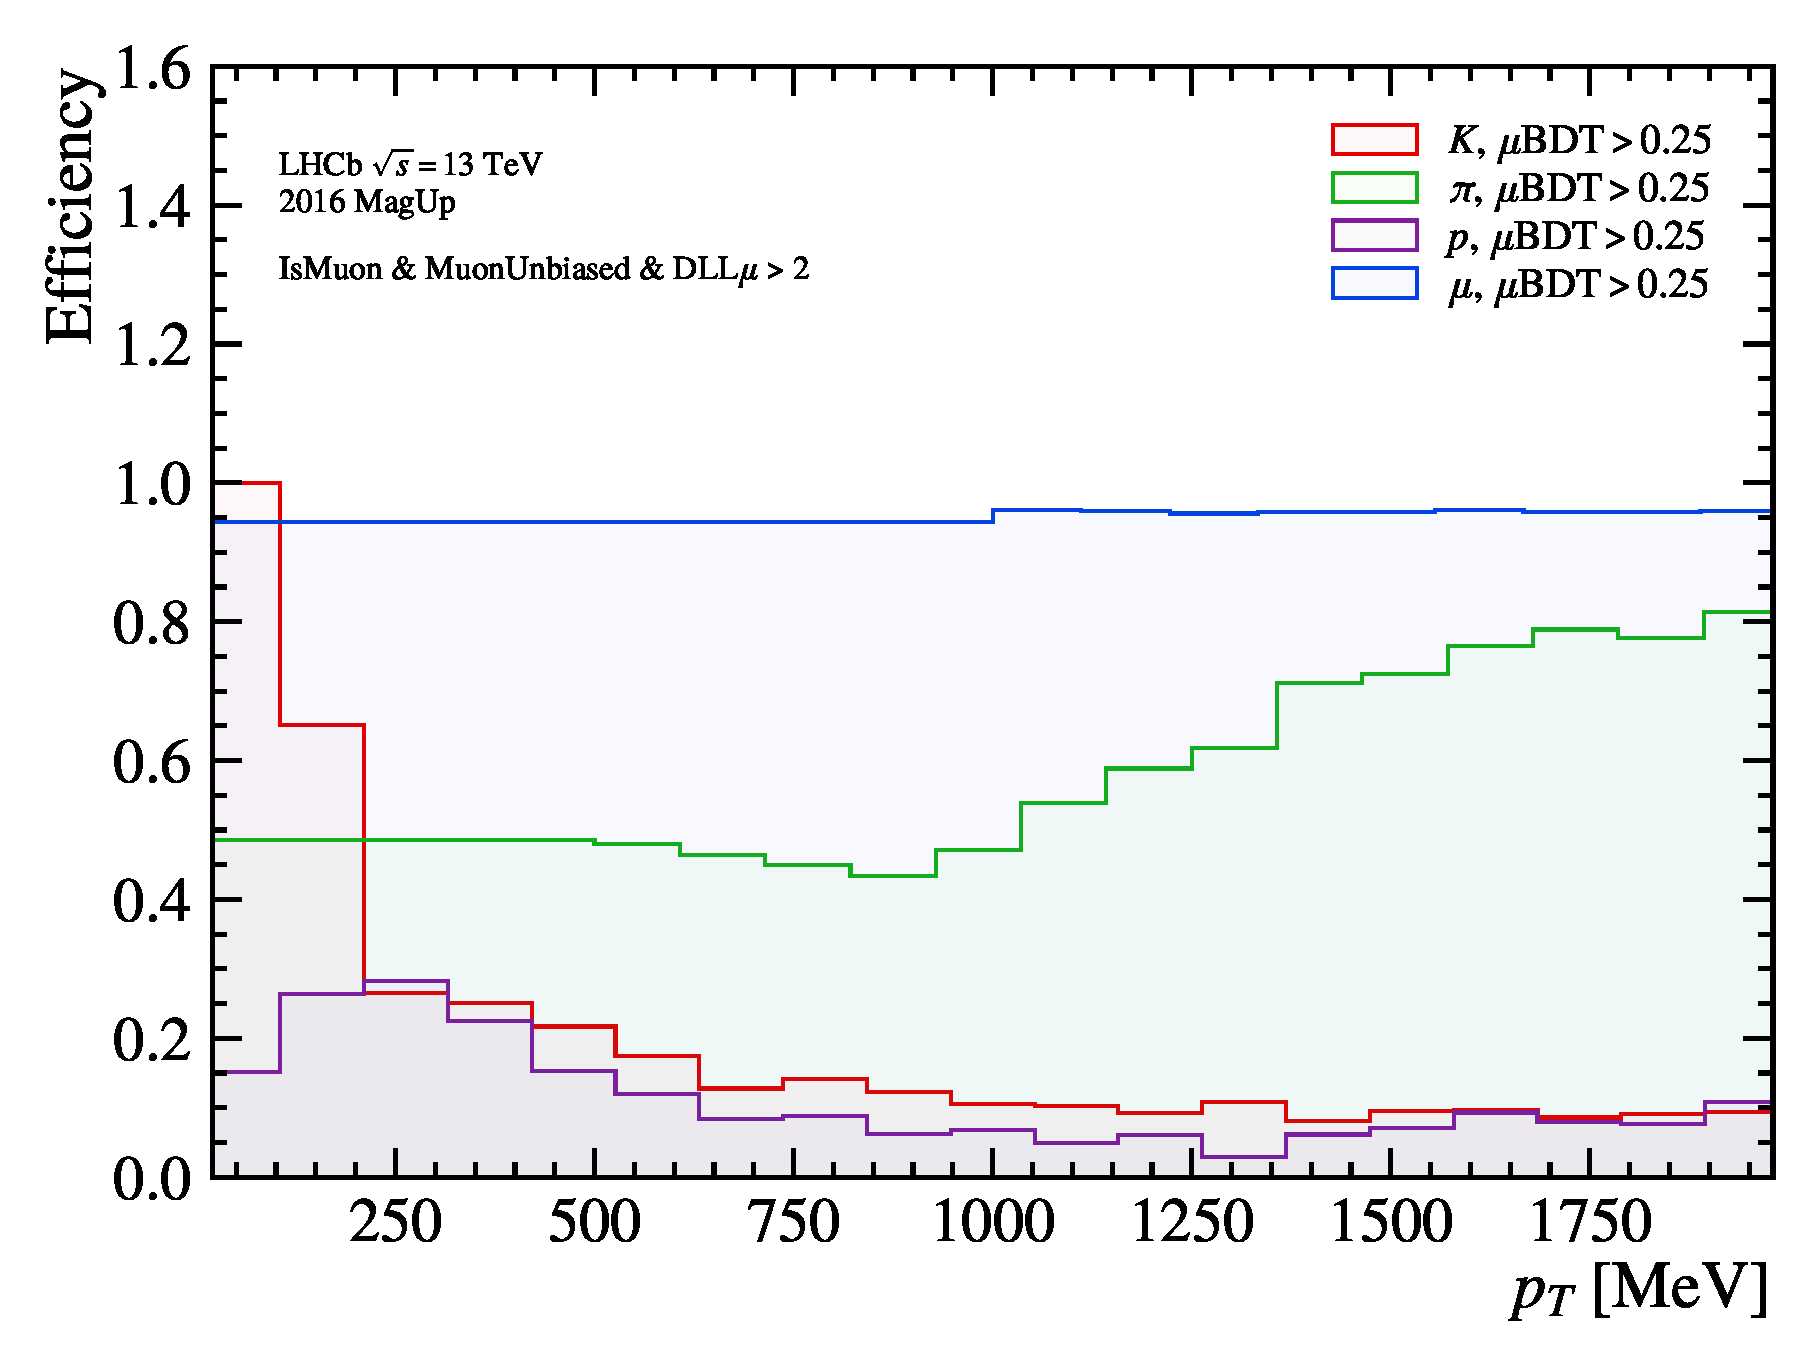
\includegraphics[width=0.45\textwidth]{./figs-selection/eff_Brunel_PT_up_pidcalib_ubdt_eff.pdf}
%     \hspace{1em}
%     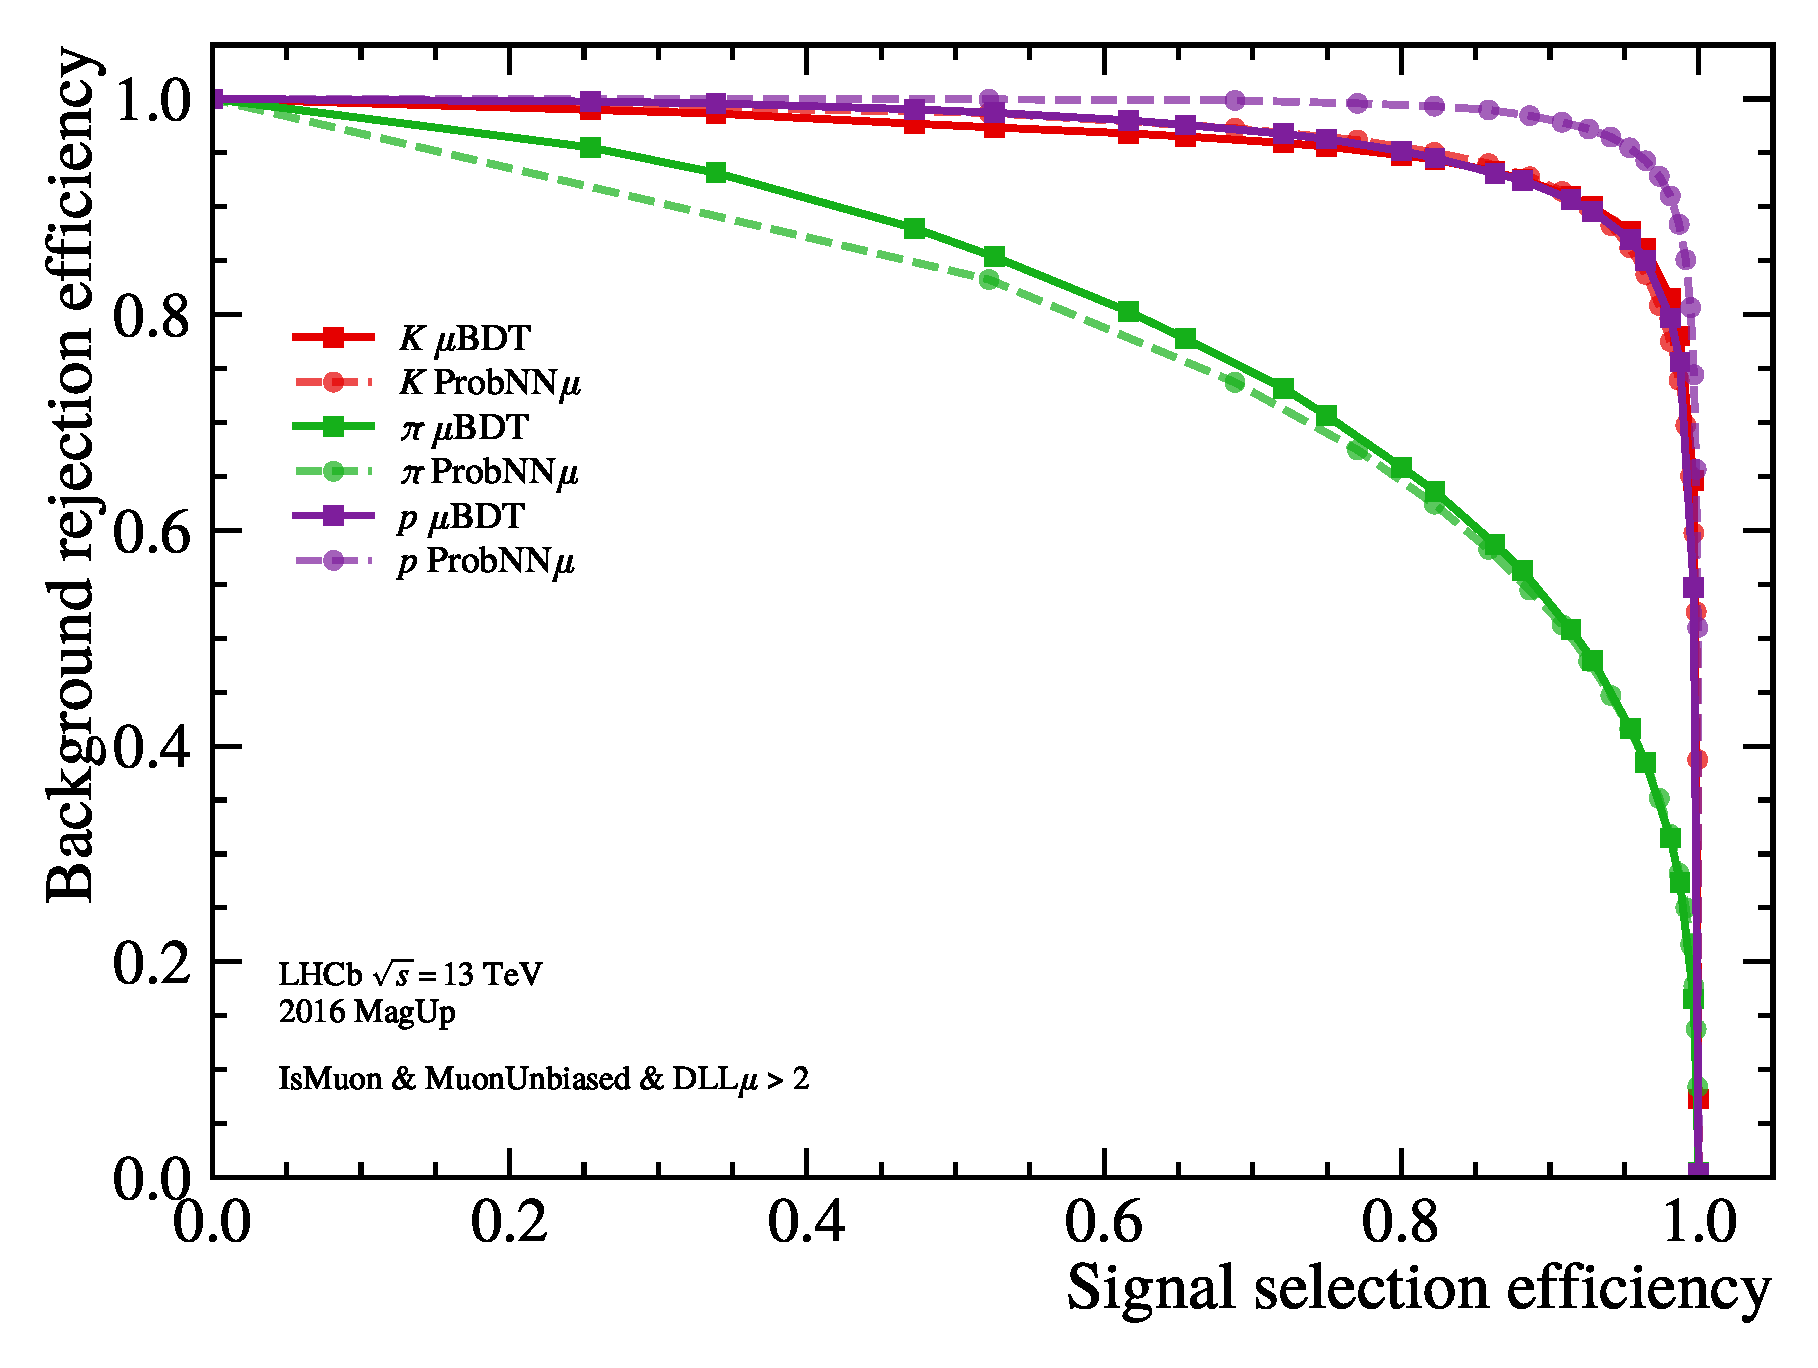
\includegraphics[width=0.45\textwidth]{./figs-selection/rej_v_eff_unbiased_Brunel_PT.pdf}

%     \caption{
%         Preliminary \UBDT study.
%         Left: \UBDT \muon selection efficiency is flat in \pt, with
%         global cut \isMuon \& $\text{\PID{\muon}}\! > 2$,
%         and $\UBDT > 0.25$.
%         Right: with the same global cut, \UBDT is more effective in rejecting
%         \pion than LHCb official \ProbNN{\muon}.
%         The \kaon rejection efficiencies are similar between the two;
%         the $p$ rejection efficiency is lower for \UBDT, but the absolute
%         rejection efficiency is high enough.
%     }
%     \label{fig:ubdt-eff}
% \end{figure}


% \section{Selected signal (ISO) and control (1OS, 2OS, DD) samples}
% \label{ref:selection:skims}

% The signal and control samples are selected by inspecting if there exists
% additional charged tracks that are compatible with coming from the
% reconstructed \B vertex.
% To predict the possibility of a charged track originating from the \B vertex,
% a multivariate BDT, referred as ``isolation BDT'', is used.
% The BDT is conceptually identical to the one used in
% \cite{LHCb-ANA-2020-056} but with the BDT re-trained based on LHCb run 2
% simulation.

% The isolation BDT\footnote{
%     The isolation BDT can be found at
%     \techurllink{https://github.com/umd-lhcb/TupleToolSemiLeptonic/blob/master/Phys/TupleToolSemiLeptonic/src/TupleToolApplyIsolation.cpp}{github/umd-lhcb/TupleToolSemiLeptonic}.
% } is added to the \davinci reconstruction sequence.
% It loops over all charged tracks in the event\footnote{
%     More specifically, these tracks are coming from
%     \texttt{StdAllNoPIDsPions}, \texttt{StdNoPIDsUpPions},
%     and \texttt{StdNoPIDsVeloPions}.
% },
% providing isolation scores for each of them where
% higher score implies higher probability of coming from the vertex, named as
% ``anti-isolated''.
% Three tracks with highest isolation scores\footnote{
%     The ones that are most likely to be anti-isolated.
% } are saved in the output file, in descending order\footnote{
%     So the first one is the most anti-isolated one among all charged tracks
%     in the event.
% }.

% Below a brief description for the signal sample and the main physics background
% control samples is provided.
% The actual isolation selections are listed in \cref{tab:skim-cut}.

% \begin{itemize}
%     \item ISO: $B \rightarrow D^{(*)} \lepton \neulb$, with $\lepton \in \{\muon,
%         \tauon\}$.
%         This is referred as signal, or ``isolated'', sample.
%         It requires that no additional charged track is from the \B vertex
%         (in a probabilistic sense, with probability related to the isolation
%         score)
%         and is compatible with a fully reconstructed \B decay
%         (ignoring missing neutrino(s)).

%     \item DD: $B \rightarrow D^{(*)}D X$,
%         with dominate $D \rightarrow \Kp \mun \neumb X$ sub-decays.
%         This is a double-charm ($DD$) control sample,
%         which is selected by requiring at least one anti-isolated track,
%         a \kaon-like long track\footnote{
%             This means the track went through both upstream and downstream
%             trackers, and is generally of good tracking quality.
%         } and a hard track in the three most anti-isolated tracks\footnote{
%             Note that these three requirements can be satisfied by a single
%             track.
%         }.

%     \item 1OS: $B \rightarrow D^{**} \lepton \neulb$.
%         This control sample, enriched in excited charm states,
%         requires one and only one additional anti-isolated charged long track
%         that is compatible with a \pion PID hypothesis and has correct charge
%         for a $D^{**} \rightarrow D^{(*+)}\pim$ decay.

%     \item 2OS: $B \rightarrow D^{**}_H \lepton \neulb$,
%         where $H$ stands for ``heavy''.
%         This control sample is enriched in highly excited (heavy) charm states,
%         which is selected by requiring two and only two anti-isolated \pion-like
%         long tracks of opposite charge,
%         capable of $D^{**}_H \rightarrow D^{(*)} \pip\pim$ decay.

%         % Why?
%         This sample also provides an independent selection of
%         $B \rightarrow D^{(*)}D X$ backgrounds, where the \pip\pim fit into the
%         $X$ category and \kaon escapes isolation detection.
% \end{itemize}

% \begin{table}[htb]
%     \caption{Signal and control sample isolation requirements.}
%     \label{tab:skim-cut}
%     \centering
%     \begin{tabular}{c|rll}
%         \toprule
%         {\bf Sample}  & {\bf Variable}              & {\bf Cuts}     \\
%         \midrule
%         ISO           & \isoBDT{1}                  & $< 0.15$       \\
%         \midrule
%         1OS           & \isoBDT{1}                  & $> 0.15$       \\
%                       & \isoBDT{2}                  & $< 0.15$       \\
%                       & \isoTrack{1}                & $= 3$\parnote{
%                           This means a long track.
%                       }                                              \\
%                       & $p_1$                       & $> 5$ GeV      \\
%                       & $p_{T,1}$                   & $> 0.15$ GeV   \\
%                       & \ProbNN{$K_1$}              & $< 0.2$        \\
%                       & $Q_1 \cdot \text{PID}_\Dz$\parnote{
%                           Apply to \Dz channel,
%                           which implies that the anti-isolated \pip can
%                           form a \Dstarp with the \Dz.
%                       }                             & $> 0$          \\
%                       & $Q_1 \cdot \text{PID}_\Dstar$\parnote{
%                           Apply to \Dstar channel.
%                           Here it is required that the anti-isolated \pim can
%                           form a $D^{**0}$ with the \Dstarp.
%                       }                             & $< 0$          \\
%         \midrule
%         2OS           & \isoBDT{1}                  & $> 0.15$       \\
%                       & \isoBDT{2}                  & $> 0.15$       \\
%                       & \isoBDT{3}                  & $< 0.15$       \\
%                       & \isoTrack{1}                & $= 3$          \\
%                       & \isoTrack{2}                & $= 3$          \\
%                       & {\footnotesize
%                          Max$(p_1 \cdot (p_{T,1} > 0.15 \text{ GeV}),
%                               p_2 \cdot (p_{T,2} > 0.15 \text{ GeV}))$
%                         }
%                                                     & $> 5$ GeV      \\
%                       & \ProbNN{$K_1$}              & $< 0.2$        \\
%                       & \ProbNN{$K_2$}              & $< 0.2$        \\
%                       & $Q_1 \cdot Q_2$             & $< 0$          \\
%         \midrule
%         DD            & \isoBDT{1}                  & $> 0.15$       \\
%                       & {\footnotesize$\begin{aligned}
%                             \text{Max}(
%                             &p_1 \cdot (p_{T,1} > 0.15\text{ GeV}),  \\
%                             &p_2 \cdot (p_{T,2} > 0.15\text{ GeV})
%                                  \cdot (\text{\isoBDT{2}} > -1.1),   \\
%                             &p_3 \cdot (p_{T,3} > 0.15\text{ GeV})
%                                  \cdot (\text{\isoBDT{3}} > -1.1)
%                             )
%                         \end{aligned}$}             & $> 5$ GeV      \\
%                       & Max(\ProbNN{$K_{1,2,3}$})   & $> 0.2$        \\
%                       & \isoTrack{\text{the one passing $K$ PID requirement}}
%                                                     & $= 3$          \\
%                       & \isoBDT{\text{the one passing $K$ PID requirement}}
%                                                     & $> -1.1$       \\
%         \bottomrule
%     \end{tabular}
%     \begin{flushleft}
%         \parnotes
%     \end{flushleft}
% \end{table}


% \section{Veto of overlapping candidates}
% \label{ref:selection:veto}

% % See this note: https://github.com/umd-lhcb/rdx-run2-analysis/blob/master/docs/cuts/Dst_veto_in_D0.md
% % TODO: The number need to be updated
% Since the reconstruction of a \Dstar\muon pair always requires the existence
% of a \Dz\muon pair,
% there is about 35\% of events in the signal sample of the \Dstar
% channel leaks into \Dz channel.
% This is likely due to the fact that slow \pion typically has poor tracking
% resolution (small \ipChiSq), making the \Dz\pion vertex of poor quality which
% makes the reconstruction fail and \Dstar partially reconstructed as \Dz.

% To veto the overlapping candidates between \Dz and \Dstar channel,
% a tool\footnote{
%     Named \texttt{TupleToolApplyIsolationVetoDst}, which can be found at
%     \techurllink{https://github.com/umd-lhcb/TupleToolSemiLeptonic/blob/master/Phys/TupleToolSemiLeptonic/src/TupleToolApplyIsolationVetoDst.cpp}{github/umd-lhcb/TupleToolSemiLeptonic}
% }.
% is added to the \davinci reconstruction sequence, which processes all tracks
% in the event with the following procedure:

% \begin{enumerate}
%     \item Denote the track as $t$
%     \item Refit a vertex from \Dz and $t$.
%     \item Compute $\Delta m_\text{veto} \equiv m_{\Dz t} - m_\Dz$
%     \item Test if $\Delta m_\text{veto} \in [140~\text{GeV}, 160~\text{GeV}]$.
%         If it is, record $\Delta m_\text{veto}$ and the isolation BDT
%         score of this track.
% \end{enumerate}

% From all recorded BDT scores and $\Delta m_\text{veto}$, the
% $\Delta m_\text{veto}$ of the tracks with top two BDT scores are saved.
% It is then filtered offline (listed in \cref{tab:offline-cut-d0})
% that these two tracks,
% the best slow \pion candidates,
% are \emph{incompatible} with
% forming a \Dz\pion vertex with a mass close to \Dstar PDG mass.

% Note that this tool does not rank tracks based \emph{solely} on the isolation,
% because the poor tracking resolution of the slow \pion implies that the track is
% \emph{not guaranteed} to have a large isolation score, as it maybe more
% compatible to be originating from PV, instead of the \B vertex.
% Ranking tracks that fall within the $[140~\text{GeV}, 160~\text{GeV}]$
% mass window based on their BDT scores
% makes the veto procedure more robust, as reported in \cite{LHCb-ANA-2020-056}.

% In addition, an alternative mass hypothesis is tested
% (offline, also listed in \cref{tab:offline-cut-d0}), where the reconstructed
% \muon is treated as a \pion,
% and $\Delta m_\text{alt hypo} = m_{\Dz\muon_\text{as \pion}} - m_\Dz$
% is computed\footnote{
%     By using the 3-momentum of the \muon, while using $m_\pion$ as the invariant
%     mass of the track.
% } and required to be inconsistent with \Dstar PDG mass.

% The veto procedures are applied on all samples of the \Dz channel only.
